\subsection{UC17 - Visualizzazione risultato ricerca prodotto}
\begin{figure}[H]
  \centering
  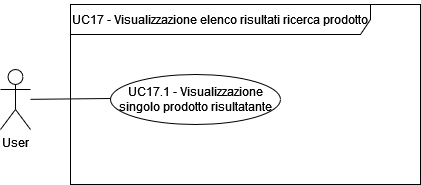
\includegraphics[width=0.8\textwidth]{UC_diagrams_11-20/UC17.drawio.png}
   \caption{Diagramma UML UC17 - Visualizzazione risultato ricerca prodotto}
\end{figure}
\begin{itemize}
    \item \textbf{Attori:} User.
    \item \textbf{Pre-condizione:} L'utente ha ricercato un prodotto [UC16].
    \item \textbf{Post-condizione:} Il prodotto risultante dalla ricerca viene selezionato [UC15].
    \item \textbf{Scenario Principale:} L'utente, dopo aver ricercato un determinato nome, visualizza il prodotto corrispondente che verrà automaticamente selezionato.
    \item \textbf{Generalizzazioni:} -
    \item \textbf{Estensioni:} -
\end{itemize}